\documentclass{beamer}
\usetheme{Antibes}

\usepackage{amsfonts}
\usepackage{amssymb}
\usepackage{amsmath}
\usepackage{amsthm}

% My commands
\newcommand{\R}{\mathbb{R}}
\newcommand{\N}{\mathbb{N}}
\newcommand{\Z}{\mathbb{Z}}
\newcommand{\T}{\mathrm{T}}
\newcommand{\E}{\mathbb{E}}
\newcommand{\Var}{\mathrm{Var}}
\newcommand{\Cov}{\mathrm{Cov}}
\newcommand{\Dcal}{\mathcal{D}}

\newtheorem{proposition}{Proposition}

\title[Decision-dependent DRO]{
	Decision-dependent Distributionally Robust Optimization
}
\subtitle{
	The Facility Location Problem with Random Demand
}
\author[Fortin-Leblanc, Joshaghani]{
	Gabriel Fortin-Leblanc\inst{1} \and Mohammad Joshaghani\inst{2}
}
\institute{
	\inst{1}
	Université de Montréal
	\and
	\inst{2}
	Université du Québec à Montréal
}
\date{November 29, 2024}

\begin{document}
	
	\frame{\titlepage}
	
	\begin{frame}{Outline}
		\tableofcontents
	\end{frame}
	
	\section{Introduction to the problem} % Gabriel ~ 3 min.
	\begin{frame}[allowframebreaks]
		\begin{columns}
			\column{0.4\textwidth}
			\begin{itemize}
				\item Different capacities
				\item Different opening costs
				\item Transportation fees
				\item Opened facilities affect the demand
			\end{itemize}
			Which facilities to open so the cost is minimized?
			
			\column{0.7\textwidth}
			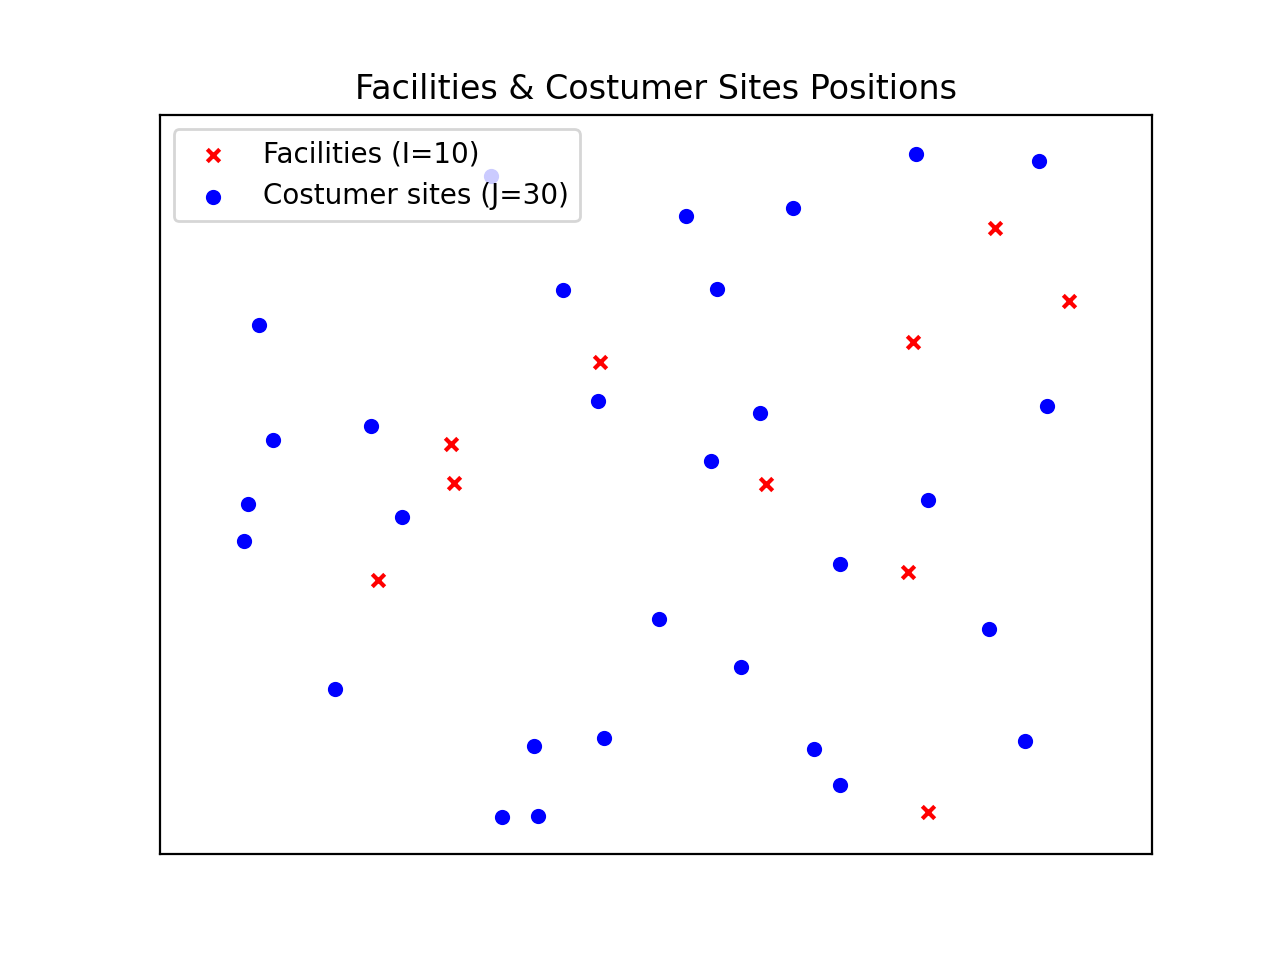
\includegraphics[width=\textwidth]{../figure/facility_costumer_site_pos.png}
		\end{columns}
		
		\framebreak
		\begin{itemize}
			\item $J$ costumer sites
			\item $I$ possible location for facilities
			\item $y \in \{0, 1\}^I$ the decision variables
			\item $O \in \R_+^{I}$ the opening costs
			\item $C \in \R_+^{I}$ the capacities
			\item $t \in \R_+^{I \times J}$ the transportation fees
			\item $\Dcal = \{\xi_k \in \R_+: k \in [K]\}$ the support of the demand (same for each costumer sites)
			\item $d(y) \in \Dcal^J$ the random demand
			\item $r \in \R_+^{J}$ the revenues
			\item $p \in \R_+^{J}$ the penalty for not responding to the demand
		\end{itemize}
		
		\framebreak
		\begin{definition}[The model]
			For some value $y \in \{0, 1\}^{I}$, let
			\begin{equation*}
				U(y) \subset \left\{\pi \in \R_+^{J \times K}: \pi 1_K = 1_J\right\}
			\end{equation*}
			be a set of distribution over the demand for each customer sites. The \textbf{robust counterpart of a facility location problem (FLP)} is
			\begin{equation} \label{eq:outterproblem}
				\min_{y \in \{0, 1\}^I} \left\{O^\T y + \max_{\pi \in U(y)} \E h(y, d(y))\right\},
			\end{equation}
		\end{definition}
		\framebreak
		\begin{definition}[The model]
			where
			\begin{subequations}
				\label{eq:innerproblem}
				\begin{align}
					h(y, d(y)) = \min_{x, s} &\sum_{i \in I} \sum_{j \in J} t_{ij}x_{ij} + \sum_{j \in J} (p_j s_j - r_j d_j(y)) \\
					\text{s.t.} &\sum_{i \in I} x_{ij} + s_j = d_j(y) \quad \forall j \in [J] \\
					&x_{ij} \le C_i y_i \quad \forall i \in [I], j \in [J] \\
					&s_i, x_{ij} \ge 0 \quad \forall i \in [I], j \in [J].
				\end{align}
			\end{subequations}
		\end{definition}
	\end{frame}
	
	\section{Derive a finite-dimensional MILP} % Gabriel ~ 7 min.
	\begin{frame}
		\begin{enumerate}
			\item Retrieve a one-level minimization.
			\item Linearize bilinear and trilinear terms.
		\end{enumerate}
	\end{frame}
	
	\subsection{Finite-dimensional Problem}
	\begin{frame}[allowframebreaks]
		Steps for obtaining a one-level minimization:
		\begin{enumerate}
			\item Use the duality theorem with the inner Problem \ref{eq:innerproblem} to obtain a maximization problem.
			\item Combine the maximum from the duality to the maximum of the Problem \ref{eq:outterproblem}.
			\item Use the duality theorem with the combined maximization problem to obtain a minimization problem.
		\end{enumerate}
		
		\framebreak
		\begin{proposition}
			% TODO: Proposition 1
		\end{proposition}
		
		\framebreak
		\begin{proposition}
			% TODO: Theorem 1
		\end{proposition}
	\end{frame}
	
	\subsection{Linearized Problem}
	\begin{frame}
		% TODO
	\end{frame}
	
	\section{Thight the constraints for better convergence} % Mohammad ~ 4 min.
	\begin{frame}
		% TODO: Describe the new valid contraints
	\end{frame}
	
	\section{Experiments} % Mohammad ~ 3 min.
	\begin{frame}
		% TODO: Present the results of the experiment
	\end{frame}
	
	\section{What more?} % ~ Mohammad 3 min.
	\begin{frame}
		% TODO: Present the improvments to come
	\end{frame}
\end{document}